%==============================================================================
% Sjabloon poster bachproef
%==============================================================================
% Gebaseerd op document class `a0poster' door Gerlinde Kettl en Matthias Weiser
% Aangepast voor gebruik aan HOGENT door Jens Buysse en Bert Van Vreckem

\documentclass[a0,portrait]{hogent-poster}


% Info over de opleiding
\course{Bachelorproef}
\studyprogramme{toegepaste informatica}
\academicyear{2022-2023}
\institution{Hogeschool Gent, Valentin Vaerwyckweg 1, 9000 Gent}

% Info over de bachelorproef
\title{\Huge Scholieren met dyslexie van de derde graad middelbaar onderwijs ondersteunen bij het begrijpend lezen van wetenschappelijke artikelen via gepersonaliseerde ATS.}

\subtitle{}
\author{Dylan Cluyse}
\email{dylan.cluyse@student.hogent.be}
\supervisor{Lena De Mol}
\cosupervisor{Johan Decorte (Hogeschool Gent); Jana Van Damme (Hogeschool Gent)}

% Indien ingevuld, wordt deze informatie toegevoegd aan het einde van de
% abstract. Zet in commentaar als je dit niet wilt.
\specialisation{AI en data engineering}
\keywords{Gepersonaliseerde tekstvereenvoudiging; dyslexie; natuurlijke taalverwerking}
\projectrepo{https://github.com/dylancluyse/bachelorproef-nlp-tekstvereenvoudiging}

\begin{document}

\maketitle

\begin{abstract}
Ingewikkelde woordenschat en zinsbouw hinderen scholieren met dyslexie in de derde graad van het middelbaar onderwijs bij het begrijpend lezen van wetenschappelijke artikelen. Gepersonaliseerde \textit{manual text simplification} (MTS) helpt deze scholieren bij hun leesbegrip. Daarnaast kan \textit{automatic text simplification} (ATS) dit proces automatiseren om de werkdruk bij leraren en scholieren te verminderen. Dit onderzoek achterhaalt met welke technologische en logopedische aspecten AI-ontwikkelaars rekening moeten houden bij de ontwikkeling van een AI-toepassing voor geautomatiseerde en gepersonaliseerde tekstvereenvoudiging. Hiervoor stelt het onderzoek de volgende onderzoeksvraag op: "Hoe kan een wetenschappelijk artikel automatisch worden vereenvoudigd, gericht op de unieke noden van scholieren met dyslexie in de derde graad middelbaar onderwijs?". Een requirementsanalyse achterhaalt de benodigde functionaliteiten om gepersonaliseerde ATS mogelijk te maken. Vervolgens wijst de vergelijkende studie uit welk taalmodel ontwikkelaars kunnen inzetten om de taak van gepersonaliseerde en geautomatiseerde tekstvereenvoudiging mogelijk te maken. De requirementsanalyse wijst uit dat toepassingen om wetenschappelijke artikelen te vereenvoudigen, gemaakt zijn voor een centrale doelgroep en geen rekening houden met de unieke noden van een scholier met dyslexie in de derde graad middelbaar onderwijs. Toepassingen voor gepersonaliseerde ATS zijn mogelijk, maar ontwikkelaars moeten meer inzetten op de unieke noden van deze scholieren.
\end{abstract}

\begin{multicols}{2} % This is how many columns your poster will be broken into, a portrait poster is generally split into 2 columns

\section{Introductie}

% Zin uit script nemen --> in inleiding
% 'vindt u deze zin moeilijk om te lezen'


% Tweede filmpje bekijken
% voor- en na
% cumuleerbare

\begin{quotation}
\textit{Ikwkgndeleie worechnsadot en zinsdouw hdirnnen scholieren met dlyixsee in de drdee graad middeldaar onberwijs bij het lezen van wkieclnphtjaepese ateirkeln.}
\end{quotation}

Vindt u deze zin moeilijk te lezen? Dit kan voor scholieren met dyslexie dagelijkse kost zijn bij het begrijpend lezen. Stoort het vakjargon en veel informatie in een compact formaat u bij het begrijpend lezen van nieuw wetenschappelijk onderzoek? Dit is niet abnormaal, want het begrijpend lezen van wetenschappelijke artikelen vraagt een alsmaar grotere geletterdheid van de lezer. Toch kunnen leerkrachten deze hindernis voor de studenten verwerpen, door teksten met \textit{manual text simplification} (MTS) te vereenvoudigen. Om de werkdruk in het onderwijs tegen te gaan, moet dit proces ook geautomatiseerd worden met \textit{automated text simplification} (ATS). Figuur \ref{img:onderzoeksvragen} illustreert de centrale onderzoeksvraag, gekoppeld aan de deelvragen die het onderzoek moet beantwoorden.

% Alle doelgroepen krijgen het moeilijk te verduren, maar scholieren met dyslexie ervaren hier een nog grotere hindernis mee.  

\begin{center}
	\captionsetup{type=figure}
	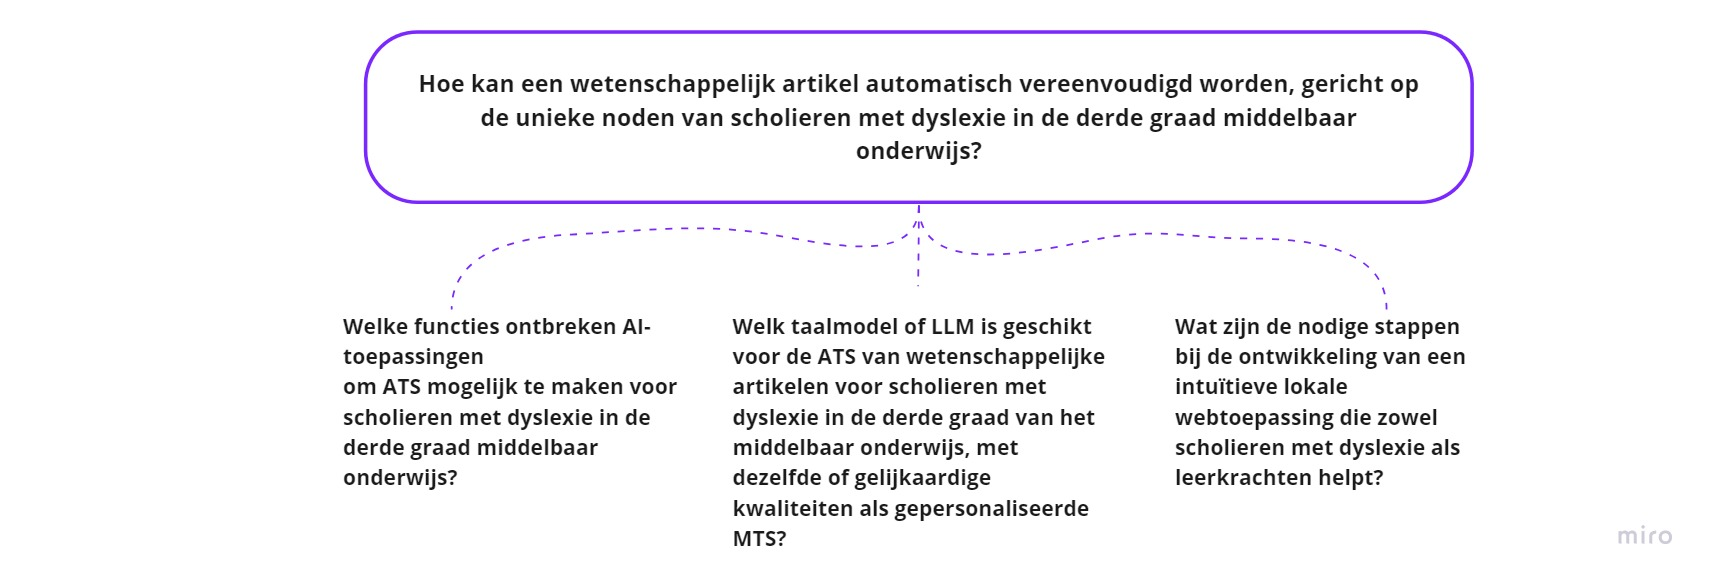
\includegraphics[width=1.0\linewidth]{figures/onderzoeksvragen.jpg}
	\captionof{figure}{Centraal de onderzoeksvraag.}
	\label{img:onderzoeksvragen}
\end{center}

\section{Onderzoeksmethoden}

Om een werkwijze te achterhalen voor het ontwikkelen van dergelijk toepassing, voert het onderzoek drie fasen uit weergegeven op figuur \ref{img:flowchart}. 

De requirementsanalyse toetst de huidige toepassingen af op hun MTS-functionaliteiten. 

De vergelijkende studie van taalmodellen gebeurt met machinale en menselijke beoordeling. Het onderzoekt laat de machine op basis van leesbaarheidsscores en het aantal (complexe/lange) woorden per zin. Daarnaast maakt het onderzoek gebruik van referentieteksten vereenvoudigd door leerkrachten en scholieren om de gelijkenissen en gebreken te achterhalen van ATS-teksten met MTS-teksten.



\begin{center}
	\captionsetup{type=figure}
	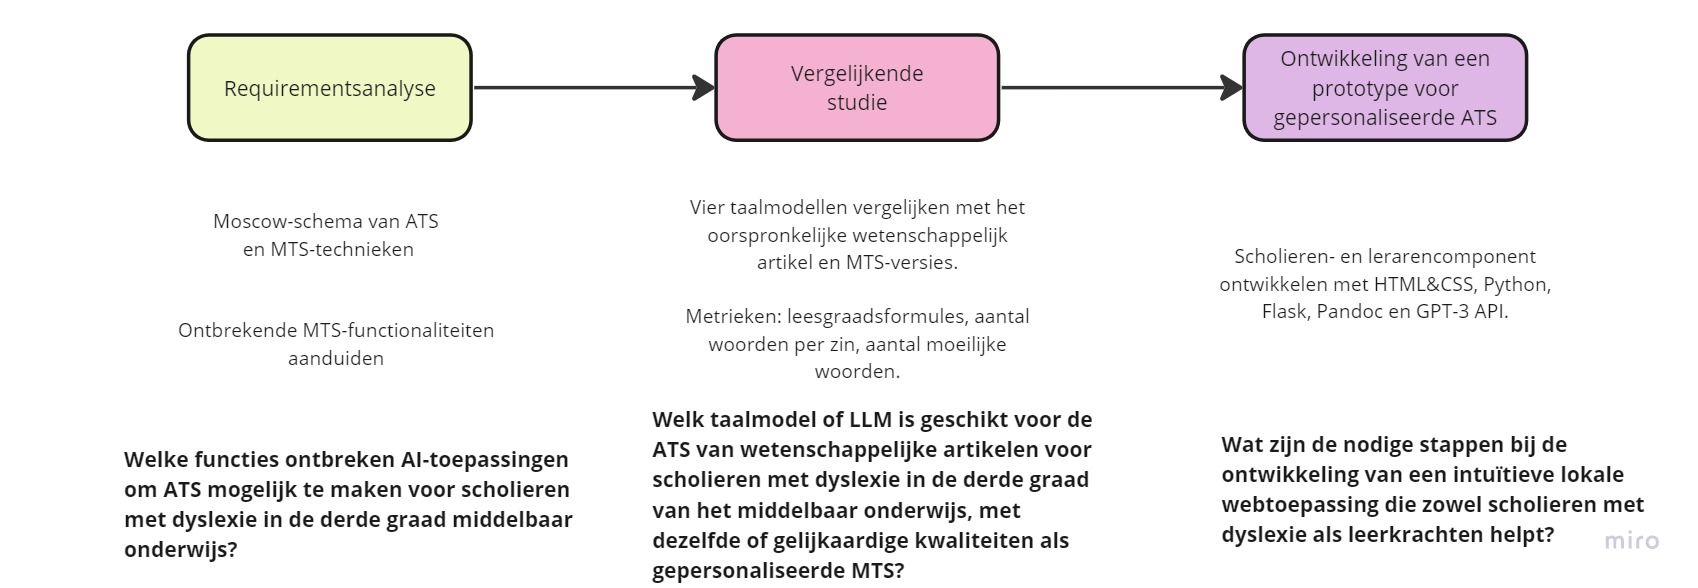
\includegraphics[width=1.0\linewidth]{figures/onderzoeksmethoden.jpg}
	\captionof{figure}{De gebruikte onderzoeksmethoden. In het vetgedrukt staan de onderzoeksvragen beschreven.}
	\label{img:flowchart}
\end{center}

\section{Resultaten}

Scholieren kunnen de tekst aanpassen. Daarnaast kunnen leerkrachten een vereenvoudigde versie van een wetenschappelijk artikel laten maken met het prototype. Hier kan de leerkracht parameters meegeven, waaronder de opmaakopties en de vereenvoudigingen die de tekst moet aannemen.

\section{Conclusies}

Uit de requirementsanalyse blijkt dat bestaande online tools en softwaretoepassingen voor ATS onvoldoende gepersonaliseerde functionaliteiten bieden. Ze missen opmaakopties voor scholieren met dyslexie. Recente technologieën bieden wel tekstvereenvoudigingsopties, maar vereisen informaticakennis die de meeste scholieren en leraren niet hebben. Een vergelijkende studie toont aan dat het GPT-3 taalmodel geschikt is voor LS en SS-technieken, terwijl andere taalmodellen minder coherente tekst genereren. Het prototype voor gepersonaliseerde ATS maakt gebruik van AI en NLP-technologieën zoals PDFMiner, de GPT-3 API en Pandoc. Hoewel het prototype nog niet aan alle functionaliteiten voldoet, kunnen ontwikkelaars met de gebruikte softwarepakketten een volledig afgewerkte toepassing ontwikkelen. Figuur \ref{img:verder-onderzoek} toont de verdere onderzoeksonderwerpen aan.
% Verder onderzoek naar de toepassing van AI via een API, zoals het GPT-4 taalmodel, is noodzakelijk en kan baanbrekend zijn voor de onderwijssector. Dit onderzoek kan zich richten op doelgroepinschattingen via prompts en het potentieel van de combinatie van GPT-3 en \textit{full-text-search}-technologieën. Daarnaast is er behoefte aan onderzoek naar de verschillen tussen taalmodellen getraind op wetenschappelijke artikelen en taalmodellen getraind op algemene data. Tot slot kunnen logopedisten en studenten in deze richting het prototype gebruiken om verder onderzoek uit te voeren naar de effecten van gepersonaliseerde ATS bij scholieren met dyslexie in de derde graad van het middelbaar onderwijs. 

\begin{center}
	\captionsetup{type=figure}
	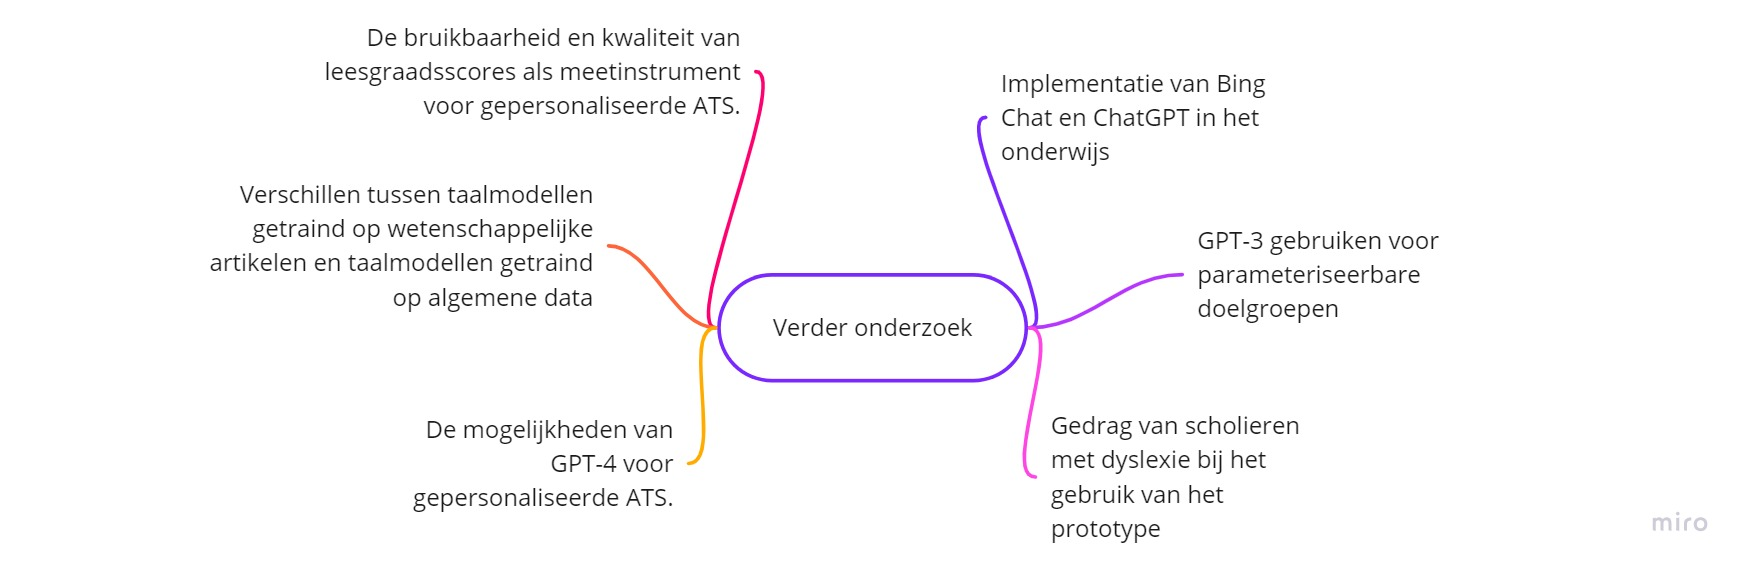
\includegraphics[width=1.0\linewidth]{figures/verder-onderzoek.jpg}
	\captionof{figure}{}
	\label{img:verder-onderzoek}
\end{center}

\end{multicols}
\end{document}